\documentclass[../main.tex]{subfiles}
\graphicspath{{../images/}}

\begin{document}
\subsection*{Lecture 21: \hfill  3/18/24}
\hrule \vspace{10px}
\section{Non-inertial Frames}
In the \emph{noninertial} frame, N1L and N2L do not hold true. In the simplest example of an
accelerating frame, we have simple pendulum in a car moving in a straight line with velocity $\vb V$ and acceleration
$\dot{\vb V} = \vb A$. In the lab frame (inertial),$\mathcal{S}_0$, we can relate the position of the
moving frame $\mathcal{S}$ by
\begin{align*}
    \dot{\vb r}_0 &= \dot{\vb r} + \vb V \\ 
    \ddot{\vb r}_0 &= \ddot{\vb r} + \vb A \\
    \implies &\ddot{\vb r}_0 &= \ddot{\vb r} - \vb A
\end{align*}
so N2L in $\mathcal{S}_0$ is always
\begin{align*}
    \vb F &= m \ddot{\vb r}_0 = m (\ddot{\vb r} - \vb A)
\end{align*}
so in the noninertial frame, $\mathcal{S}$, we have
\begin{align*}
    m\ddot{\vb r} &= F - m\vb A
\end{align*}
The procedure of mechanics in noninertial frames is as follows:
\begin{enumerate}
    \item write down equations in lab frame using $\vb r_0$
    \item identify coordinates in noninertial frame
\end{enumerate}
So in $\mathcal{S}$ we have an effective gravity
\begin{align*}
    m\ddot{r} &= m\vb g - m \vb A \\
    &= m \vb g_{\text{eff}}
\end{align*}
where the trigonometry tells us
\begin{align*}
    \tan\phi_0 = \frac{A}{g}
\end{align*}
so we have a new equation of motion
\begin{align*}
    \ddot \theta = -\frac{g_{\text{eff}}}{L} \sin(\theta - \theta_0)
\end{align*}
where
\begin{align*}
    g_{\text{eff}} = \sqrt{g^2 - A^2}
\end{align*}
with frequency
\begin{align*}
    \omega &= \sqrt{\frac{g_{\text{eff}}}{L}}
\end{align*}
the force in the noninertial frame
\begin{align*}
    F_{NI} &= -m\vb A
\end{align*}
is known as the inertial or \emph{fictitious} force. From before we know that the gravitational force
is actually
\begin{align*}
    F_g &= -\frac{G m_1 m_2}{r^2} \vu r \\
    &= m \vb g \qquad \vb g = - \frac{GM_E}{R_E^2} \vu r
\end{align*}
where we assume a constant gravity near the surface of the Earth.

\paragraph*{Einsteins Equivalence Principle} Einstein thought that gravitational mass equals
inertial mass. Thus Gravity is a fictitious force.

\paragraph*{Tidal Forces} Without considering the earth rotating on its axis or orbiting the sun, we
can see that it is in a noninertial frame due to the gravitational attraction of the moon! So this
lab frame (or God Frame as we must consider ourselves external to the motion of the earth) the 
N2L tells us
\begin{align*}
    m \ddot{\vb r_0} &= m \vb g - \frac{G M_m m}{d^2} \vu d + \vb F_{ext}
\end{align*}
and in the noninertial frame we have
\begin{align*}
    \vb A = -\frac{G M_m}{d_0^2} \vu d_0
\end{align*}
so N2L is
\begin{align*}
    m\ddot r = m\vb g - \frac{G M_m m}{d^2} \vu d + \vb F_{ext} + \frac{G M_m m}{d_0^2} \vu d_0
\end{align*}
we call this difference of forces due to the moon the \emph{tidal force}:
\begin{align*}
    m\ddot r = m \vb g + \vb F_{ext} + \vb F_{\text{tid}} \\
    \vb F_{\text{tid}} = -GM_m m \qt(\frac{\vu d}{d^2} - \frac{\vu d_0}{d_0^2})
\end{align*}
so on the far side of the earth (furthest from the moon) we have $d^2 < d_0^2$ so the tidal force
points away from the moon. On the near side of the earth, the tidal force points towards the moon.
we can also see that the tidal force is equivalent to the difference in gravitational force of the
moon on the object minus the force of the moon at the center of mass of the earth. Earth as an
extended object is subject to tidal forces, and applies to all extended objects such as black holes.

For example the tidal forces of a dinosaur near a black hole would strech and compress the dinosaur.

\newpage
\subsection*{Lecture 22: \hfill 3/20/24}
\paragraph*{Rotating Reference Frame} 

What is rotation? u.r.t an axis i.e. angular velocity $\vb \omega$ where the direction of the vector
is the axis and magnitude is the speed of rotation $\omega$. To determine the direction of rotation
we use the Right Hand Rule. 

\paragraph*{Euler's Theorem} The most general motion of a body about a fixed point is also a
rotation about an axis that passes through the fixed point.

Common Notation:
\begin{itemize}
    \item $\vb \Omega$ is a fixed angular velocity
    \item $\vb \omega$ is a specific (unknown) angular velocity.
\end{itemize}
From Taylor Figure 9.7, we can see that the distance from the point from the rotating axis $\rho$ 
gives the relation $\rho = r \sin\theta$. And the magnitude of velocity is
\begin{align*}
    \nu = \omega \rho = \omega r \sin\theta
\end{align*}
and hence the velocity
\begin{align*}
    \vb \nu = \vb \omega \times \vb r = \dot{\vb r}
\end{align*}
So in general, the time derivative of a vector in a rotating frame is always in the form
\begin{align*}
    \dot{\vb u} = \omega \times \vb u
\end{align*}
\paragraph*{Rotating Frame} From last time, we have the to frames of reference:
\begin{itemize}
    \item $\mathcal{S}_0$ the lab frame (God frame)
    \item $\mathcal{S}$ the rotating frame
\end{itemize}
Where $\Omega$ is the angular velocity of $\mathcal{S}$ in $\mathcal{S}_0$.
\paragraph*{} For a rotation about the Earth we have
\begin{align*}
    \Omega = \frac{2\pi}{24 \times 3600} \sim \qty{7.3e-5}{rad\per\s}
\end{align*}
In $\mathcal{S}$ we define coordinate basis vectors
\begin{align*}
    \vu e_1,\; \vu e_2,\; \vu e_3
\end{align*}
Which are orthogonal, and in $\mathcal{S}_0$, $\vu e_i$ rotates with ang. velocity $\vb \Omega$.

\paragraph*{} Goal: Write N2L in $\mathcal{S}$.

In $\mathcal{S}_0$ we have N2L
\begin{align*}
    m\ddot{\vb r}_0 = \vb F
\end{align*}
For a general vector
\begin{align*}
    \vb Q = Q_1 \vu e_1 + Q_2 \vu e_2 + Q_3 \vu e_3 = \sum_i Q_i \vu e_i
\end{align*}
In the rotating frame the change in unit vectors are constant
\begin{align*}
    \dot{\vu e}_i &= 0 \qqtext{in} \mathcal{S} \\
    \implies \dot{\vu e}_i &= \vb \Omega \times \vu e_i \qqtext{in} \mathcal{S}_0
\end{align*}
So
\begin{align*}
    \qt(\dv{\vb Q}{t})_{\mathcal{S}} &= \sum_i \dv{Q_i}{t} \vu e_i \\
    \qt(\dv{Q}{t})_{\mathcal{S}} &= \sum_i \dv{Q_i}{t} \vu e_i + \sum Q_i \dot{\vu e}_i
\end{align*}
And in the lab frame
\begin{align*}
    \qt(\dv{\vb Q}{t})_{\mathcal{S}_0} &= \sum_i \dv{Q_i}{t} \vu e_i + \sum Q_i \vb \Omega \times \vu e_i \\
    &= \qt(\dv{\vb Q}{t})_{\mathcal{S}} + \vb \Omega \times \vb Q
\end{align*}
So N2L in the lab frame is
\begin{align*}
    m \qt(\dv[2]{\vb r}{t})_{\mathcal{S}_0} &= \vb F \\
    \qt(\dv{t})_{\mathcal{S}_0} \qt(\dv{\vb r}{t})_{\mathcal{S}_0} &= 
        \qt(\dv{t})_{\mathcal{S}_0} 
        \qt[\qt(\dv{\vb r}{t})_{\mathcal{S}} + \vb \Omega \times \qt(\dv{\vb r}{t})_{\mathcal{S}}] \\
    &= \qt(\dv{t})_\mathcal{S} \qt[
        \qt(\dv{\vb r}{t})_\mathcal{S} + \Omega \times \vb r
    ]
    + \Omega \times \qt[
        \qt(\dv{\vb r}{t})_\mathcal{S} + \Omega \times \vb r
    ] \\
    &= \qt(\dv[2]{\vb r}{t})_\mathcal{S} + 2\Omega \times \qt(\dv{\vb r}{t})_\mathcal{S} 
        + \Omega \times (\Omega \times \vb r)
\end{align*}
where we let
\begin{align*}
    \dot{\vb r} = \qt(\dv{\vb r}{t})_\mathcal{S}
\end{align*}
which we can rewrite the N2L as
\begin{align*}
    \vb a_{\mathcal{S}_0} &= \ddot{\vb r} + 2 \vb \Omega \times \dot{\vb r} 
        + \vb \Omega \times (\vb \Omega \times \vb r)
\end{align*}
SO the N2L in the lab frame is simply
\begin{align*}
    m \vb a_{\mathcal{S}_0} = \vb F
\end{align*}
and in the rotating frame we have
\begin{align*}
    m(\ddot{\vb r} &+ 2\vb \Omega \times \dot{\vb r} + \vb \Omega \times (\vb \Omega \times \vb r)) = \vb F \\
    m\ddot{\vb r} &= \vb F - 2m\vb \Omega \times \dot{\vb r} - m\vb \Omega \times (\vb \Omega \times \vb r) \\
    &= \vb F + 2m \dot{\vb r} \times \vb \Omega + m(\vb \Omega \times \vb r) \times \vb \Omega \\
    &= \vb F + \vb F_{\text{cor}} + \vb F_{\text{cf}}
\end{align*}
where we have two extra terms: the Coriolis force and a Centrifugal force. 

\paragraph*{Coriolis Force} From the Centrifugal force
\begin{align*}
    \vb F_{\text{cf}} &= m (\vb \Omega \times \vb r) \times \vb \Omega \\
    \vb F_{\text{cf}} &= m \vb v \times \vb \Omega \\
    F_{\text{cf}} &= m v \Omega = m \rho \Omega^2 \\ 
    &= \frac{m \rho^2 \Omega^2}{\rho} = \frac{m v^2}{r}
\end{align*}
\paragraph*{Example: St Louis} The colatitude of St Louis is $\theta = \qty{51.4}{\degree}$ so
using
\begin{align*}
    \Omega_E = \qty{7.3e-5}{rad\per\s} \quad R_E \approx \qty{6400}{\km} = \qty{6.4e6}{\m}
\end{align*}
we have the acceleration
\begin{align*}
    a_{\text{cf}} = (\vb \Omega \times \vb r) \times \vb \Omega = \rho \Omega^2 = r \sin\theta \Omega^2 \\
    \approx \qty{2.66e-2}{\m/\s^2}
\end{align*}
and since we know that the acceleration due to Earth
\begin{align*}
    a_g = \frac{GM_E}{r^2}
\end{align*}
and using
\begin{align*}
    G = \qty{6.67e-11}{\m^3\kg^{-1}\s^{-2}} \quad M_E = \qty{5.9e24}{\kg} \\
    r_{eq} \approx \qty{6378}{\km} \quad r_{pole} \approx \qty{6356}{\km}
\end{align*}
the change in acceleration is
\begin{align*}
    \Delta a_g &= GM_E\qt(\frac{1}{r_{eq}^2} - \frac{1}{r_{pole}^2}) \\
    &\approx \qty{6.8e-2}{\m/\s^2}
\end{align*}
So we have a nonzero tangential component of acceleration due to gravity due to the rotation of the
Earth (it isn't just radial). When we look at the acceleration of the Earth orbiting the sun we find
\begin{align*}
    a_{\text{orbit}} \sim \qty{6.0e-3}{\m/\s^2}
\end{align*}
which is only a third of the centrifugal force due to the Earth's axial rotation.

\newpage
\subsection*{Lecture 23: \hfill 3/22/24}
\paragraph*{Review:} N2L in a rotating frame:
\begin{align*}
    m\ddot{\vb r} &= \vb F + 2m \dot{\vb r} \times \vb \Omega + m(\vb \Omega \times \vb r) \times \vb \Omega \\
    &= \vb F + \vb F_{\text{cor}} + \vb F_{\text{cf}}
\end{align*}
we have an additional Coriolis force and a Centrifugal force. 

\begin{figure}[ht]
    \centering
    \captionsetup{width=0.8\textwidth}
    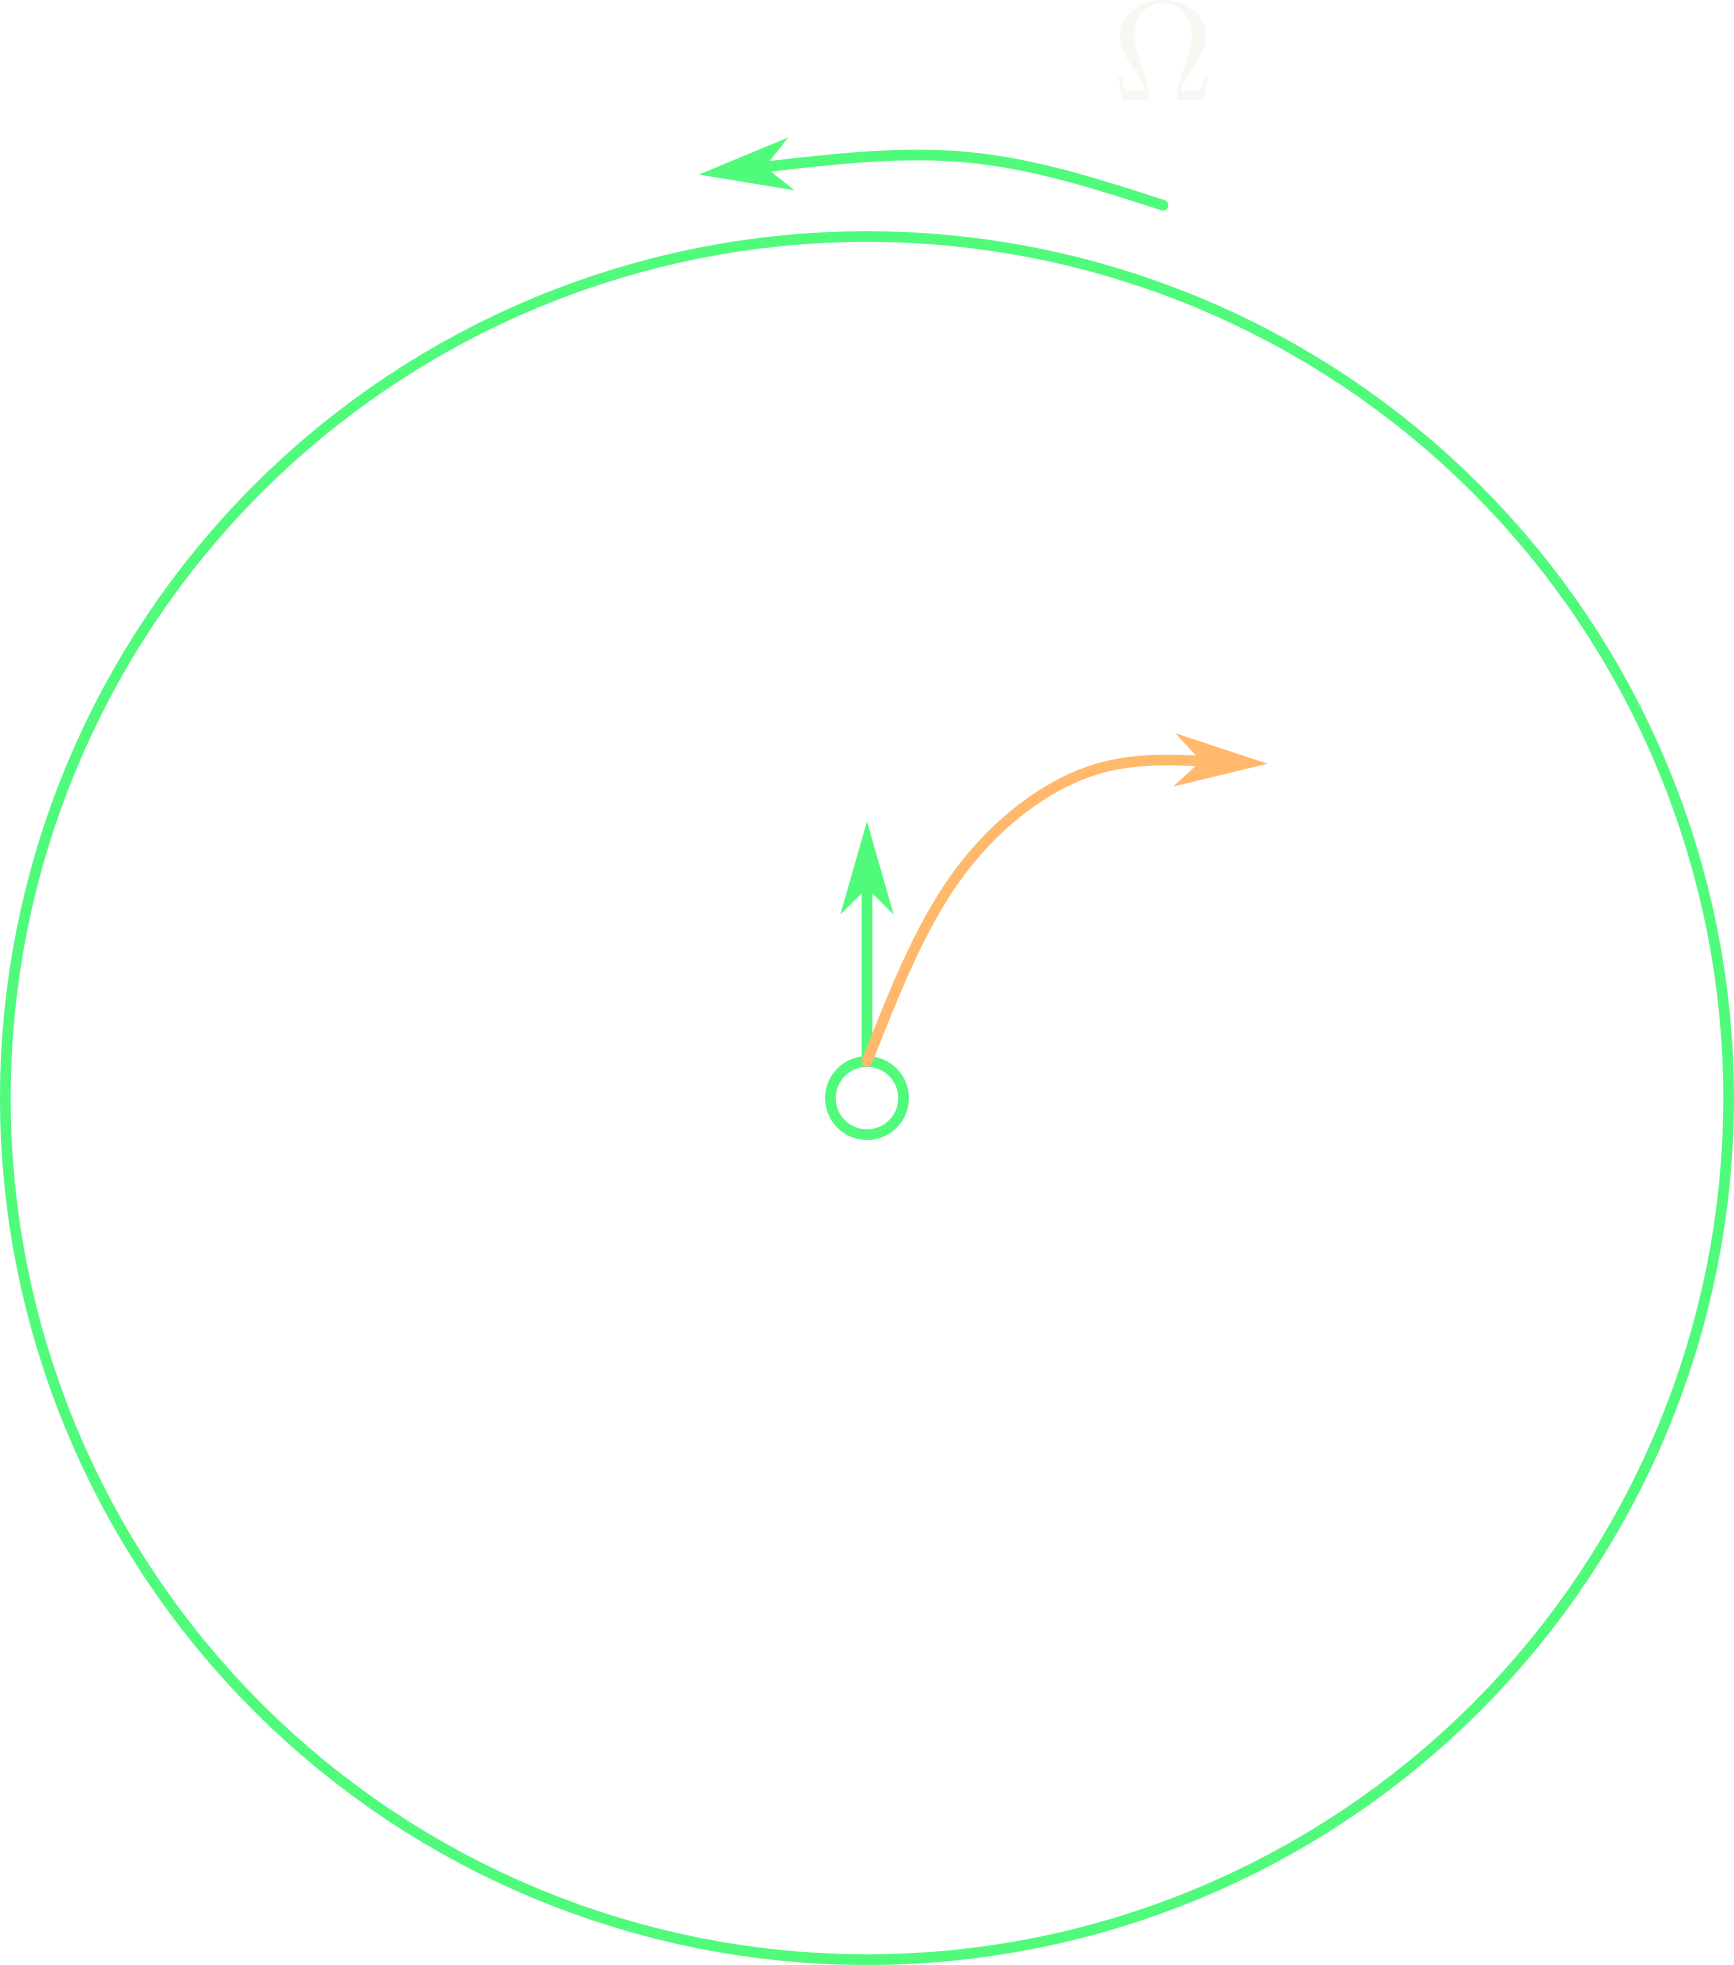
\includegraphics[width=0.4\textwidth]{turntable.png}
    \caption{Turntable with frictionless puck. In the lab frame, the puck moves in a straight line,
    but in the noninertial frame—rotating with the turntable—the puck moves in a curved path.}
\end{figure}
\subsubsection*{Coriolis Force}
\begin{align*}
    \vb F_{\text{cor}} &= 2m \dot{\vb r} \times \vb \Omega
\end{align*}
where
\begin{align*}
    \vb F_{\text{cor}} \cdot \vb v = 0
\end{align*}
when we look at the direction of the Coriolis force in the Earth's frame, at the North side the
Coriolis force points clockwise, and at the South side the Coriolis force points counterclockwise—or
the origin of cyclones. 

\paragraph*{Free Fall \& Coriolis Force} From Taylor Figure 9.15 we have the N2L in the rotating frame
\begin{align*}
    \ddot{\vb r} &= \vb g + 2 \dot{\vb r} \cross \vb \Omega
\end{align*}
where we omit the centrifugal force. We can see the vectors are
\begin{align*}
    \vb \Omega = (0, \Omega \sin\theta, \Omega \cos\theta) \\
    \vb r = (x ,y, z) \\
    \dot{\vb r} = (\dot x, \dot y, \dot z)
\end{align*}
so
\begin{align*}
    \dot{\vb r} \cross \Omega = (\dot y \Omega \cos\theta - \dot z \Omega \sin\theta, -\dot x \Omega \cos\theta, \dot x \Omega \sin\theta)
\end{align*}
and therefore using the N2L equation we have the equations of motion
\begin{align*}
    \ddot x &= 2\Omega (\dot y \cos\theta - \dot z \sin\theta) \\
    \ddot y &= -2\Omega \dot x \cos\theta \\
    \ddot z &= - g + 2\Omega \dot x \sin\theta
\end{align*}
For the 0th-order approximation we take $\Omega = 0$ and we have the simple free fall equations
\begin{align*}
    x = 0,\quad y = 0,\quad z = -\frac{1}{2}gt^2
\end{align*}
For the 1st order of rotation we substitute the 0th-order solution into the original equations:
\begin{align*}
    \ddot x &= 2\Omega \dot z \sin\theta = 2 gt \Omega \sin\theta \\
    \ddot y &= 0 \implies y = 0 \\
    \ddot z &= -g \implies z = z_0 - \frac{1}{2} gt^2
\end{align*}
where the $y$ and $z$ components are the same as the 0th-order approximation, but the $x$ equation
gives the solution
\begin{align*}
    x = \frac{1}{3} gt^3 \Omega \sin\theta
\end{align*}
\paragraph*{Example 100m Fall from St. Louis} From the vertical component we know it takes
\begin{align*}
    t = \sqrt{\frac{2z_0}{g}} \approx \qty{4.5}{\s}
\end{align*}
and we find that the object will deviate by
\begin{align*}
    \Delta x \approx \frac{1}{3} \Omega g t^3 \approx \qty{2.2}{\cm}
\end{align*}
\paragraph*{Foucault Pendulum} The equations of motion have an added Tension:
\begin{align*}
    \ddot x &= \frac{T_x}{m} + 2\Omega (\dot y \cos\theta - \dot z \sin\theta) \\
    \ddot y &= \frac{T_y}{m} - 2\Omega \dot x \cos\theta \\
    \ddot z &= \frac{T_z}{m} - g + 2\Omega \dot x \sin\theta
\end{align*}
With the $y$ pointing north and $x$ pointing east, we can see that the components of tension are 
\begin{align*}
    T_z &= T \cos\beta \\
    T_x &= T \sin\beta \cos\phi = -T \frac{x}{L} \\
    T_y &= T \sin\beta \sin\phi = -T \frac{y}{L}
\end{align*}
where $\beta \approx 0 \qquad \cos\beta \approx 1$ and $T_z \approx mg \approx T$. We can also 
assume that the pendulum is very long so $z \approx 0$ and the arc is more like a line:
\begin{align*}
    \ddot x &= -\frac{g}{L}x + 2 \dot y \Omega_z \qquad \Omega_z = \Omega \cos\theta \\
    \ddot y &= -\frac{g}{L}y - 2 \dot x \Omega_z \qquad \omega_0 = \frac{g}{L}
\end{align*}
this is a coupled system of equations 
\begin{align*}
    \ddot x - 2\Omega_z \dot y + \omega_0^2 x = 0 \\
    \ddot y + 2\Omega_z \dot x + \omega_0^2 y = 0
\end{align*}
which is solved using complex exponentials (first see Taylor 2.5):
\begin{align*}
    + i(\ddot y + 2\Omega_z \dot x + \omega_0^2 y) &= 0
\end{align*}
where
\begin{align*}
    \eta = x + iy \\
    \dot \eta = \dot x + i \dot y \\
    \ddot \eta = \ddot x + i \ddot y
\end{align*}
so adding the two equations we have
\begin{align*}
    \ddot x + i\ddot y + 2\Omega_z (\dot x + i \dot y) + \omega_0^2 (x + iy) &= 0 \\
    \ddot \eta + 2i\Omega_z \dot \eta + \omega_0^2 \eta &= 0
\end{align*}
which is a ODE from the damped harmonic oscillator with a solution $\eta \sim e^{-i\alpha t}$ where
\begin{align*}
    -\alpha^2 + 2\Omega_z \alpha + \omega_0^2 = 0 \\
    \implies \alpha = \Omega_z \pm \sqrt{\Omega_z^2 + \omega_0^2} \approx \Omega_z \pm \omega_0
\end{align*}
so we can write $\eta$ as
\begin{align*}
    \eta(t) &= C_1 e^{-(\Omega_z + \omega_0)t} + C_2 e^{-(\Omega_z - \omega_0)t} \\
    &= e^{-i\Omega_z t} (C_1 e^{-\omega_0 t} + C_2 e^{\omega_0 t}) \\
    &= e^{-i\Omega_z t} A \cos{\omega_0 t}
\end{align*}
we can see that the Foucault pendulum will rotate around the flat plane by $\Omega_z$ which is
slower than the Earth's rotation.
\end{document}